\section{Inleiding}

\subsection{Kennismaking met het vullen van vlakken}
Als introductie op deze lessenreeks over het vullen van vlakken en volumes, zullen we eens klassikaal nagaan wat dit onderwerp precies inhoudt. Om te beginnen zullen we op zoek gaan naar een goede definitie van een vlakvulling. Als we het begrip `vlakvulling' ingeven op een zoekmachine, dan vinden we een groot aantal afbeeldingen. Onder andere komen we terecht bij de volgende afbeeldingen van vlakvullingen.
\begin{figure}[h]
  \centering
  \subfloat[]{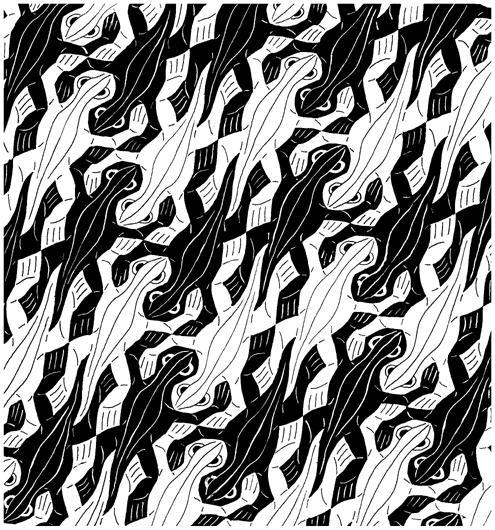
\includegraphics[height=4.8cm]{tess5}}
  \subfloat[]{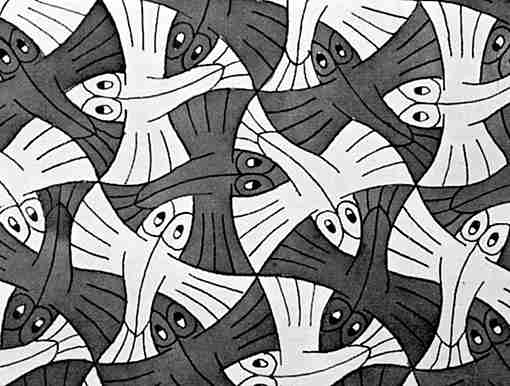
\includegraphics[height=4.8cm]{escher2}}
  \subfloat[]{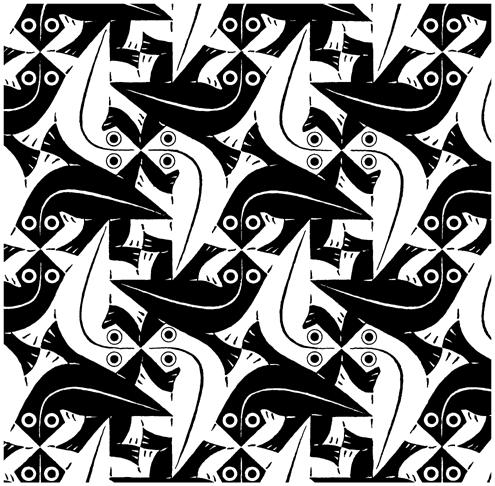
\includegraphics[height=4.8cm]{tess104}}\\
\end{figure}\\
Op deze drie afbeeldingen zien we vlakvullingen van Escher. Hier komen we later op terug.\todo{Kan jij ook ergens wat meer informatie schrijven over Escher?? Dat moet maar een paragraaf zijn, maar gewoon dat ze tenminste weten dat het een kunstenaar is!!!}\\
Nu zullen we zelf op zoek gaan naar figuren om een vlak te vullen.\\ 
\ask{Welke eenvoudige meetkundige vlakke figuren kennen jullie?}\\
\answer{Rechthoek, vierkant, driehoek, cirkel, \ldots}\\
\teacher{De leerlingen kunnen hier veel verschillende antwoorden geven, maar zullen waarschijnlijk wel komen tot de bovenstaande antwoorden.}\\
We zullen nu eens kijken hoe we een vlak volledig kunnen vullen met deze figuren aan de hand van translaties en/of rotaties. In theorie kunnen we een vlak vullen met verschillende soorten figuren, maar om het eenvoudig te houden zullen we in dit lessenpakket kijken hoe we een vlak kunnen vullen met identieke figuren.\\
\ask{Welke beperkingen moeten nog opleggen opdat iets een vlakvulling is? Als we nu het vlak willen vullen met identieke figuren mogen deze figuren dan overlappen?}\\
\teacher{Laat eerst zelf vragen en opmerkingen opkomen bij de leerlingen De leerlingen kunnen ook redeneren waarom dit zo is.}\\
Zo komen we dus tot de volgende definitie van een vlakvulling:\\
\answer{Een \textbf{vlakvulling} is een vulling van het vlak met figuren, waarbij er geen gaten mogen zijn en de figuren niet mogen overlappen.}\\
We kunnen nu proberen om een oneindig groot vlak zo optimaal mogelijk te vullen met identieke figuren.\\
\ask{Is het altijd mogelijk om een oneindig groot vlak compleet te vullen?}\\
\answer{Neen}\\
Daarom maken we dus het onderscheid tussen twee definities. Enerzijds zullen we spreken over een \textbf{complete vlakvulling} als we een oneindig vlak volledig kunnen vullen met een bepaalde figuur aan de hand van translaties en/of rotaties. Anderzijds zullen we spreken over een \textbf{optimale vlakvulling} als we het oneindig grote vlak zo compleet mogelijk kunnen vullen. Bij optimale vlakvullingen zullen we ook spreken over de \textbf{effici\"{e}ntie} van de vlakvulling. Deze effici\"{e}ntie drukken we uit in een percentage. Als de effici\"{e}ntie van de optimale vlakvulling dus gelijk is aan 100 procent, dan hebben we een complete vlakvulling.
\subsection{Vullen van een oneindig groot vlak}
Om te beginnen kunnen we nu eens kijken hoe we een vlak compleet kunnen vullen met figuren, meer bepaald zullen we proberen het vlak te vullen met regelmatige veelhoeken. Vooraleer we daarmee beginnen kunnen we eerst eens nadenken over de volgende vragen.\\
\teacher{\question{Ik vind deze indeling niet zo goed. Ik zou dus gewoon idd in groepjes werken, maar hen allemaal alle figuren geven, anders is dat megasaai!}Op dit punt verdelen we de leerlingen in 6 groepjes en delen we aan de leerlingen identieke figuren uit die uitgeknipt werden in karton. Het eerste groepje krijgt een stapel identieke regelmatige driehoeken, het tweede groepje krijgt een stapel identieke regelmatige vierhoeken, het derde groepje krijgt een stapel identieke regelmatige vijfhoeken, het vierde groepje krijgt een stapel identieke regelmatige zeshoeken, het vijfde groepje krijgt een stapel regelmatige zevenhoeken en het zesde groepje krijgt een stapel identieke regelmatige achthoeken.}\\
\task{Probeer eens uit te zoeken met welke regelmatige veelhoeken je een complete vlakvulling kan maken.}\\
\teacher{De leerlingen proberen in groepjes de tafels volledig te vullen met deze kartonnen regelmatige veelhoeken en zullen zo tot bevindingen komen.}\\
\answer{Een complete vlakvulling is enkel mogelijk met regelmatige driehoeken, regelmatige vierhoeken en regelmatige zeshoeken.}\\
\ask{Hoe komt het dat een complete vlakvulling met andere regelmatige veelhoeken niet lukt?}\\
\answer{We zien dat bij de vlakvulling met regelmatige veelhoeken de hoeken van ieder toppunt precies moeten passen omdat we anders gaten of overlappingen hebben. De grootte van de tophoeken van de regelmatige veelhoeken moet dus een deler zijn van 360.}\\
\ask{Kan je een formule vinden voor de grootte van de hoeken van een regelmatige $n-$hoek?}\\
\answer{De formule is als volgt: $180\degree-\frac{360\degree}{n}$.}\\
Als $n$ groter wordt, zien we dat de grootte van de hoeken van een regelmatige $n-$hoek nadert naar $180\degree$.\\
\teacher{We overlopen de besproken regelmatige $n-$hoeken en kijken naar de grootte van de hoeken. Hierbij worden vragen aan de leerlingen gesteld}\\
Bij een regelmatige driehoek hebben alle hoeken een grootte van \answer{$60\degree$} en \answer{$60$ is een deler van $360$}. Bij een regelmatige vierhoek hebben alle hoeken een grootte van \answer{$90\degree$} en \answer{$90$ is een deler van $360$}. Bij een regelmatige vijfhoek hebben alle hoeken een grootte van \answer{$108\degree$} en \answer{$108$ is geen deler van $360$}. Bij een regelmatige zeshoek hebben alle hoeken een grootte van \answer{$120\degree$} en \answer{$120$ is een deler van $360$}. Nu is de volgende deler van $360$ gelijk aan \answer{180}, dus \answer{er zijn geen andere $n-$hoeken waarbij we een complete vlakvulling mogelijk is}.

\todo{Wil jij ook hier net zoals in jullie Tesselatiebestand zo die figuren toevoegen waar je de vlakvulling van 3,4 en 6-hoeken ziet? Waarom heb jij het bewijs er niet in gestoken zoals in jullie bestand??!!! Met die n= 2r/(r-2)}

\subsection{Vullen van een vlak of ruimte met een welbepaalde vorm}
Anderzijds is het nu ook mogelijk om te proberen een gegeven vlak met een welbepaalde vorm te vullen met identieke figuren. We kunnen bijvoorbeeld een rechthoek met een bepaalde grootte vullen met vierkantjes of rechthoekjes of $\ldots$ Laat ons even nadenken over de volgende vragen.\\
\ask{
\begin{itemize}
\item Is het steeds mogelijk om kleine vierkantjes te vinden die een gegeven vierkant compleet opvullen?
\item Is het steeds mogelijk om kleine driehoekjes te vinden die een gegeven driehoek compleet opvullen?
\item Is het steeds mogelijk om kleine cirkeltjes te vinden die een gegeven cirkel compleet opvullen?
\end{itemize}}
\answer{Enkel het derde is niet mogelijk}
\subsection{Stapelproblemen}
Een laatste onderwerp dat we zullen bespreken in dit lessenpakket zijn de stapelproblemen. We hebben tot nu toe vooral het vullen van vlakken besproken, maar het is ook mogelijk om volumes te vullen met bepaalde voorwerpen. Opnieuw zullen we hier identieke voorwerpen kiezen om het volume te vullen. Hierbij kunnen we ons de volgende vragen stellen.\\
\ask{
\begin{itemize}
\item	Is het steeds mogelijk om kleine kubusjes te vinden die een gegeven kubus compleet opvullen?
\item Is het steeds mogelijk om kleine balkjes te vinden die een gegeven balk compleet opvullen?
\item Is het steeds mogelijk om kleine bolletjes te vinden die een gegeven bol compleet opvullen?
\end{itemize}}
\answer{Het derde is niet mogelijk}\\
We zien dus dat het niet steeds mogelijk is om een volume compleet te vullen met identieke voorwerpen. Als het mogelijk is om een gegeven volume compleet te vullen met identieke voorwerpen, dan spreken we over een \textbf{complete vlakvulling}. Anders zullen we proberen om het gegeven volume zo optimaal mogelijk te vullen. Later zullen we nog dieper ingaan op het bolstapelprobleem.
\subsection{Om over na te denken}
\ask{Ga zelf eens op zoek naar betegelingen van Escher.}\\
\ask{Kan je een voorbeeld vinden van een driehoek die gevuld is met driehoeken? \question{Op zo een vraag kan een leerling van het 4de middelbaar echt niet antwoorden denk ik.}}\\
\answer{Een voorbeeld van driehoeken in driehoeken is de driehoek van sierpinski.}\\
\teacher{Ten slotte willen we de leerlingen nog even laten verwonderd staan en laten experimenteren met enkele puzzels, tangrams of enkele raadsels rond vullen van vlakken en volumes. Dit kunnen de leerlingen in groepjes proberen oplossen.}
\begin{figure}[h]
  \centering
  \subfloat[]{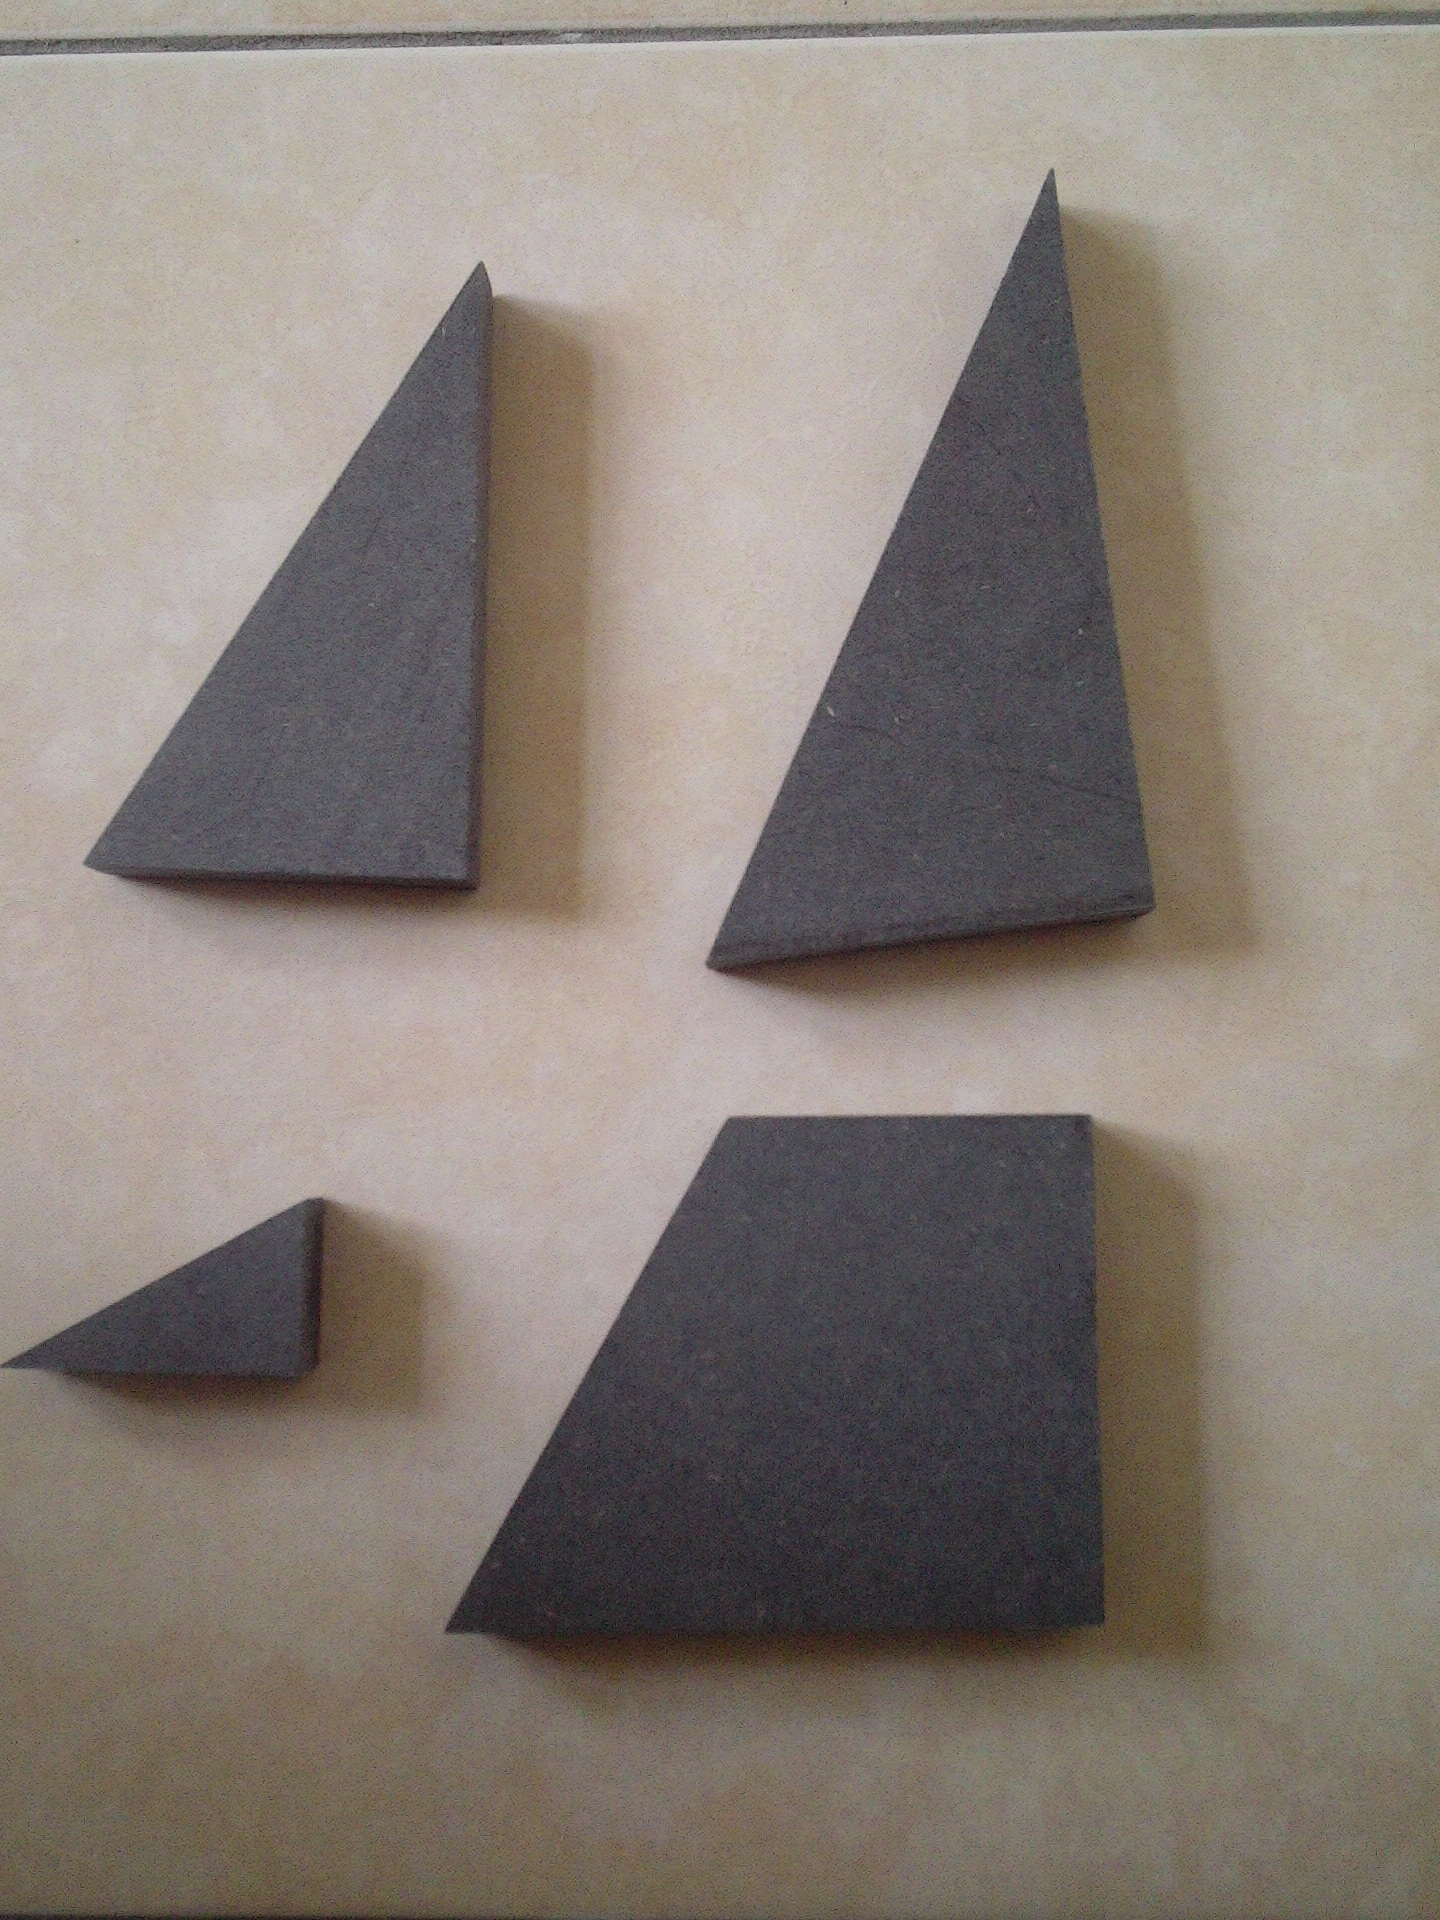
\includegraphics[height=6cm]{PIC0135}}
  \subfloat[]{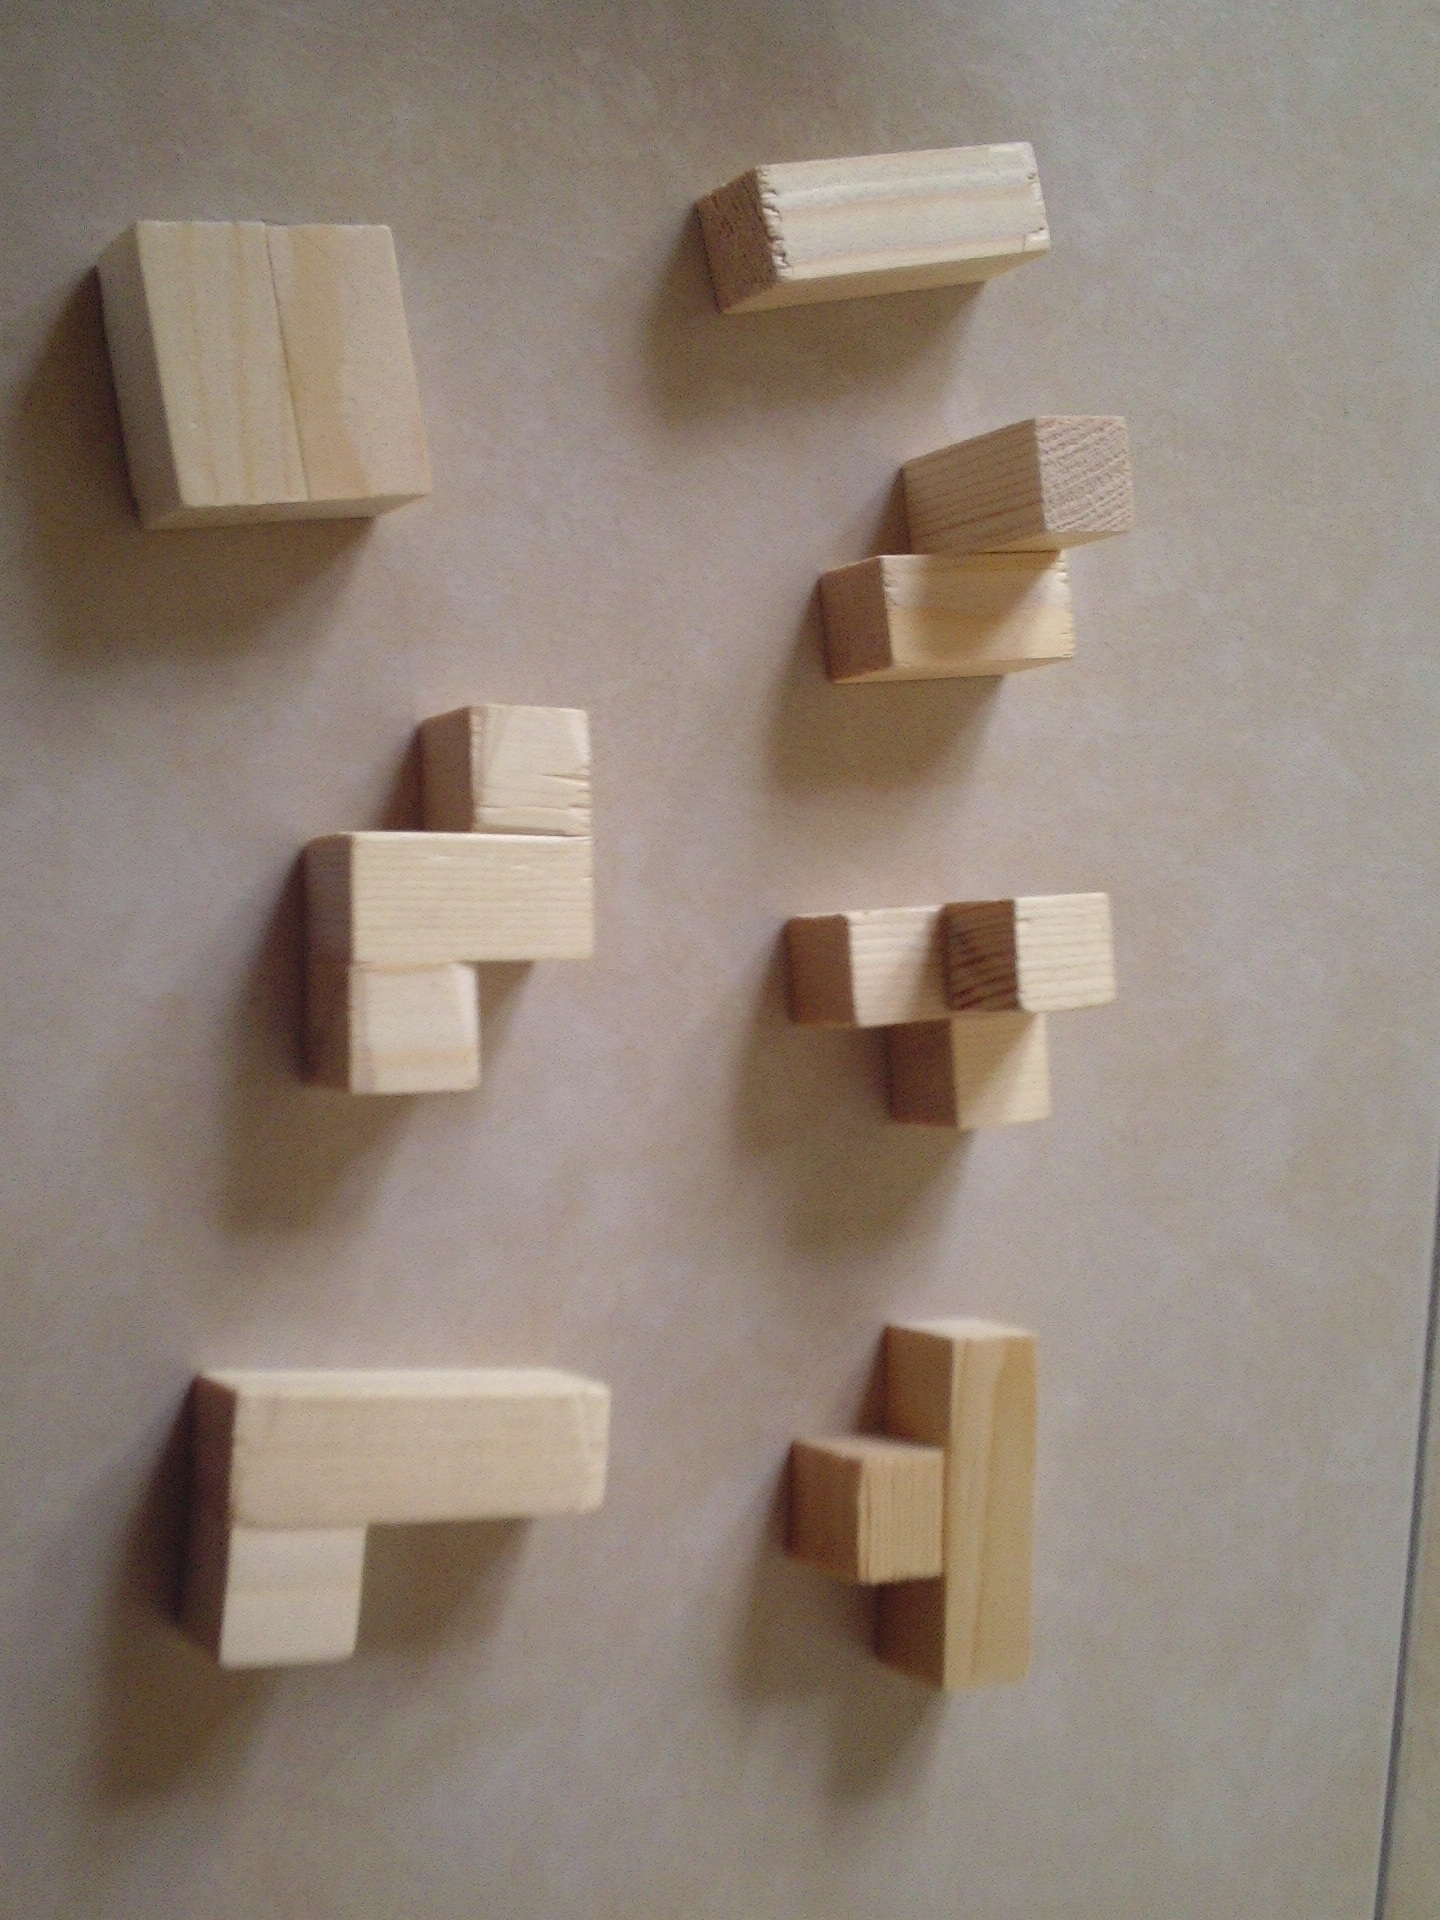
\includegraphics[height=6cm]{PIC0137}}\\
\end{figure}\\
\subsection{Wordt vervolgd}
In de volgende les zullen we ons bezighouden met het vullen van vierkanten met vierkanten. Vervolgens zal het betegelen van een vlak met zeshoeken de leidraad zijn bij het vullen van een gegeven vlak.\\
\teacher{In de eerstkomende lessen zullen we het hebben over complete vlakvullingen (les over vierkanten vullen met vierkanten en perfecte vierkanten en de les over de meetkundige interpretaties van kwadratische vergelijkingen en kubische vergelijkingen).}
